\clearpage

\subsection{Liposomal structures} ~\\
\label{plugin:vesicle}

In this section some specialized spherical multi-shell structures are summarized which describe a few types of liposomal vesicular structures. The main characteristics of a vesicle are shown in fig.\ \ref{fig:liposomal_vesicular_structure}. In first approximation these vesicles are described as spherical shell structures, where the lipid hydrophobic tail groups from the core of the spherical membrane and the hydrophilic head groups the inner and outer shell of this spherical membrane. This containment has aqueous solution inside and outside. As the lipids are in general very well known one likes to extend the models of a bilayer as described in section \ref{sect:BilayeredVesicle} or \ref{subsubsect:EllSh+SD+BiLayerGauss} by known  molecular constrains like in section \ref{subsect:DiblockCopolymerMicelles} about diblock copolymer micelles.

\begin{figure}[htb]
\begin{center}
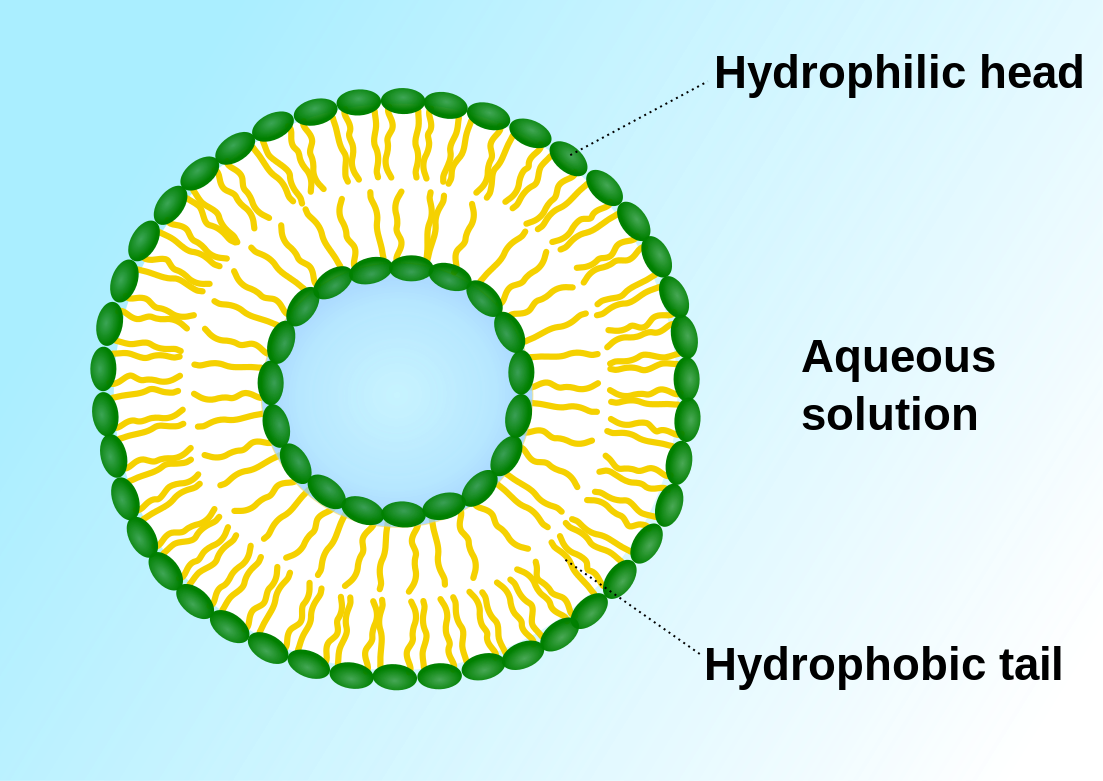
\includegraphics[width=0.8\textwidth]{../images/form_factor/vesicles/Liposome_scheme-en.png}
\end{center}
\caption{scheme of a liposomal vesicular structure}
\label{fig:liposomal_vesicular_structure}
\end{figure}

\begin{figure}[htb]
\begin{center}
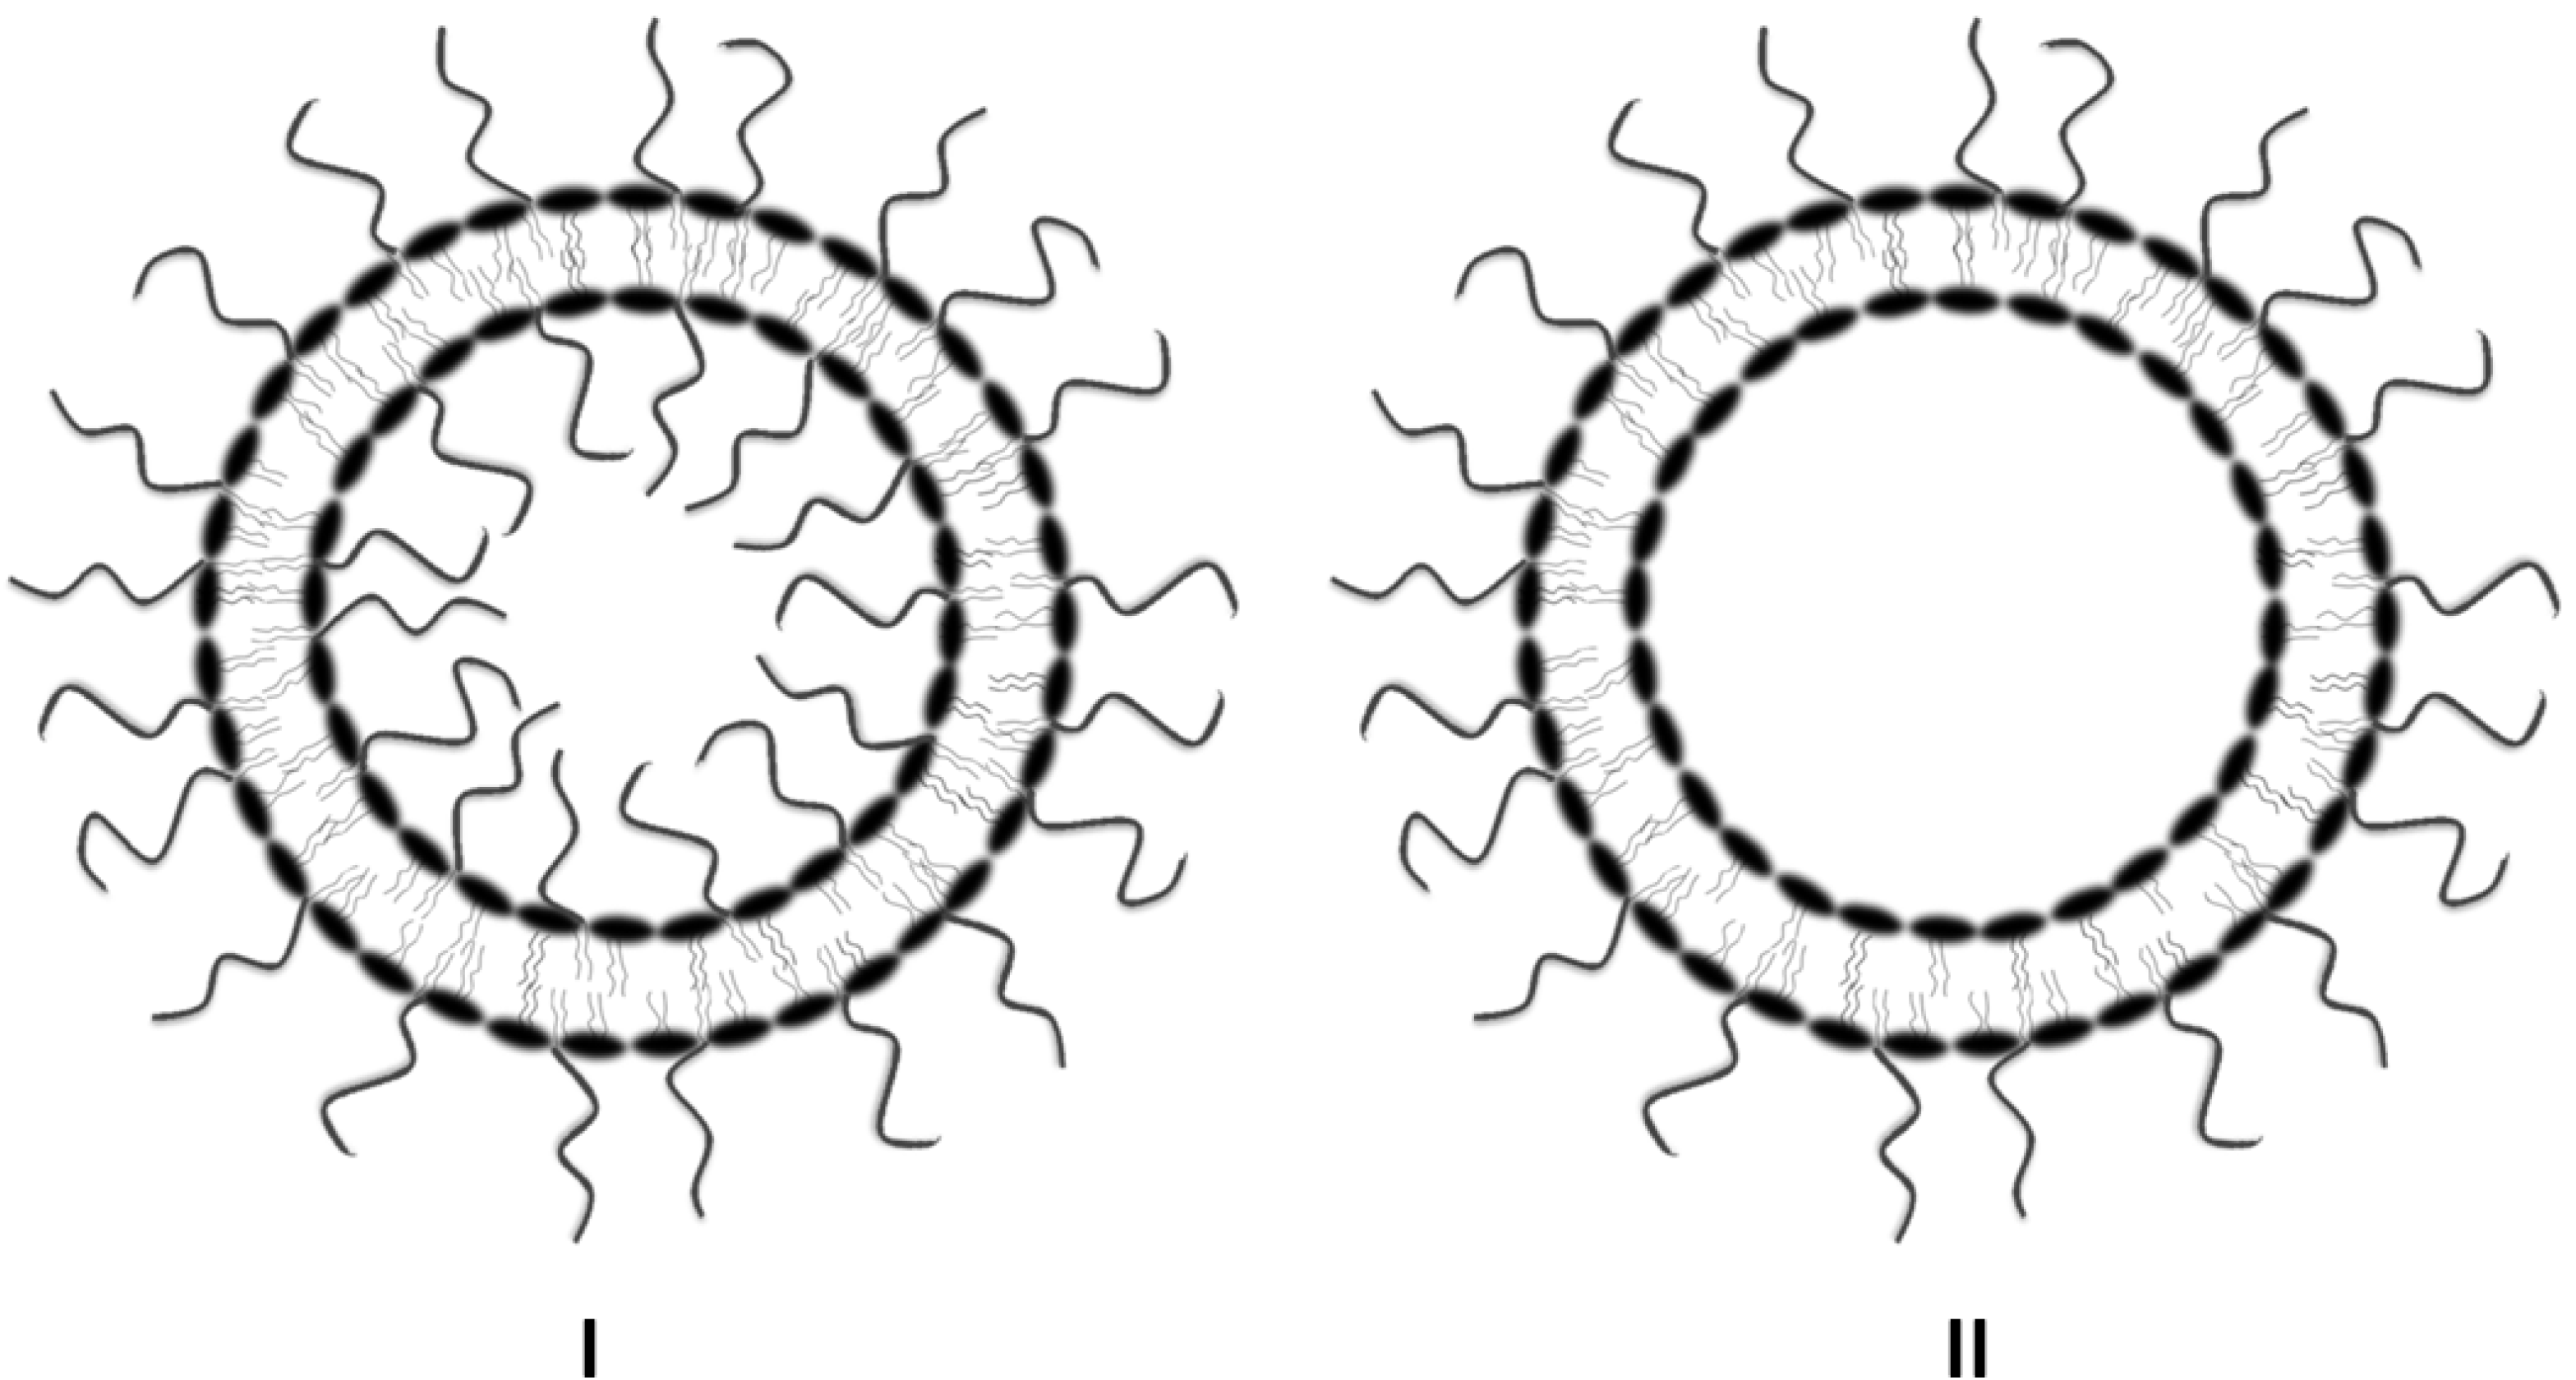
\includegraphics[width=0.8\textwidth]{../images/form_factor/vesicles/pegylated_liposome.png}
\end{center}
\caption{scheme of pegylated vesicle with PEG molecules both inside and outside or only outside the vesicle}
\label{fig:pegylated_vesicle}
\end{figure}

In pharmaceutical applications these vesicles are sometimes  decorated with PEG molecules to increase their circulation time in a living body, as they give them a sort of stealth properties against the immune system. depending on the synthesis procedure the PEG molecules are either attached on both sides or mainly from the outside as shown in fig.\ \ref{fig:pegylated_vesicle}.

The dimension in the vesicle are typically such, that the thickness of the bilayer is much smaller than the overall diameter of a micelle. Therefore next to a full 3D Fourier transform of the scattering length density profile also an approximation factorizing the contribution of the small object dimension and from the large object dimension can be performed. For very thin random orientated particles the form factor can be factorize according to Porod \cite{Porod1948} in a cross
section term $P_\text{cs}(Q)$ for the shorter or thin dimension and a shape factor $P'(Q)$ for the long dimension. For a small number of of cross-section types and shapes these functions are supplied in section \ref{plugin:Pcs4planar} and \ref{plugin:Pprime4planar}. In the cases discussed in this section knowledge about molecular properties are tried to taken into account by parameterizing the model by known molecular properties following the concept developed for block copolymer micelles \cite{PedersenGerstenberg96}.

~\\

\subsubsection{PEGylated liposome with piecewise constant bilayer scattering length density profile} ~\\

This version of a pegylated vesicle is following the formalism used in \cite{Arleth2010} and \cite{Nielsen2018}. The lipid bilayer is described in by spherical multi-shell model. Inside and outside the shell is solvent and the shell itself is formed by the lipids. The head groups point towards the solvent and the tail groups form the core like a centro-symmetric cross-section as shown in fig.\ \ref{fig:vesiclePEGpiecewconst}. The scattering intensity can be described as
\begin{align}\label{eq:vesicePEGsphsh}
  I(q) &= I_\mathrm{vv}(q) + I_\mathrm{chain}(q) + I_\mathrm{oo}(q) + I_\mathrm{ii}(q) + I_\mathrm{io}(q) +  I_\mathrm{vo}(q) + I_\mathrm{vi}(q)
\end{align}
where $I_\mathrm{vv}(q)$ is the scattering from the lipid vesicles themselves and $I_\mathrm{chain}(q)$ is the scattering from the PEG-chains alone. The next terms, $I_\mathrm{ii}(q)$ and $I_\mathrm{oo}(q)$, are the interference terms
between PEG chains attached to the inner surface of the
vesicles and between the PEG chains on the outer surface,
respectively, while $ I_\mathrm{io}(q)$ is the inter-interference between the
inner and outer PEG chains. Furthermore, the terms $I_\mathrm{vi}(q)$ and $I_\mathrm{vo}(q)$ are the interference
cross-terms of the inner and outer chains with the bilayer.
These seven terms can be written as
\begin{align}
 I_\mathrm{chain}(q) &= (n_\mathrm{i}+n_\mathrm{o})\beta_\mathrm{PEG}^2 \; 2 \frac{e^{-q^2R_g^2}-1+q^2R_g^2}{(qR_g)^4} \label{eq:vesiclePEG7chain}\\
 I_\mathrm{oo}(q) &= n_\mathrm{o}(n_\mathrm{o}-1)\beta_\mathrm{PEG}^2 \left[\frac{1-e^{-q^2R_g^2}}{q^2R_g^2}\right]^2\left[\frac{\sin\left(q(R_\mathrm{o}+H_\mathrm{o}+R_g)\right)}{q(R_\mathrm{o}+H_\mathrm{o}+R_g)}\right]^2 \label{eq:vesiclePEG7oo}\\
 I_\mathrm{ii}(q) &=  n_\mathrm{i}(n_\mathrm{i}-1)\beta_\mathrm{PEG}^2 \left[\frac{1-e^{-q^2R_g^2}}{q^2R_g^2}\right]^2\left[\frac{\sin\left(q(R_\mathrm{i}-H_\mathrm{i}-R_g)\right)}{q(R_\mathrm{i}-H_\mathrm{i}-R_g)}\right]^2 \label{eq:vesiclePEG7ii}\\
  I_\mathrm{io}(q) &= 2 n_\mathrm{i}n_\mathrm{o}\beta_\mathrm{PEG}^2 \left[\frac{1-e^{-q^2R_g^2}}{q^2R_g^2}\right]^2 \nonumber \\
  &\qquad \left[\frac{\sin\left(q(R_\mathrm{i}-H_\mathrm{i}-R_g)\right)}{q(R_\mathrm{i}-H_\mathrm{i}-R_g)}\right] \left[\frac{\sin\left(q(R_\mathrm{o}+H_\mathrm{o}+R_g)\right)}{q(R_\mathrm{o}+H_\mathrm{o}+R_g)}\right]
 \label{eq:vesiclePEG7io}\\
 F_\mathrm{sp}(q,R) &= 3\frac{\sin qR - qR\cos qR}{(qR)^3}  \\
 F_\mathrm{bi,m}(q) &= (\eta_\mathrm{h}-\eta_\mathrm{sol})\left( \frac43\pi (R_\mathrm{o}+H_\mathrm{o})^3 F_\mathrm{sp}(q,R_\mathrm{o}+H_\mathrm{o}) -  \frac43\pi R_\mathrm{o}^3 F_\mathrm{sp}(q,R_\mathrm{o}) \right) \nonumber \\
 & \qquad (\eta_\mathrm{t}-\eta_\mathrm{sol}) \left(\frac43\pi R_\mathrm{o}^3 F_\mathrm{sp}(q,R_\mathrm{o}) - \frac43\pi R_\mathrm{i}^3 F_\mathrm{sp}(q,R_\mathrm{i}) \right) \\
 & \qquad (\eta_\mathrm{h}-\eta_\mathrm{sol}) \left(\frac43\pi R_\mathrm{i}^3 F_\mathrm{sp}(q,R_\mathrm{i}) - \frac43\pi (R_\mathrm{i}-H_\mathrm{i})^3 F_\mathrm{sp}(q,R_\mathrm{i}-H_\mathrm{i})\right) \nonumber \\
 I_\mathrm{vv}(q) &= F_\mathrm{bi,m}^2(q) \label{eq:vesiclePEG7vv} \\
 I_\mathrm{vi}(q) &= 2 n_\mathrm{i}\beta_\mathrm{PEG} F_\mathrm{bi,m}(q) \frac{\sin\left(q(R_\mathrm{i}-H_\mathrm{i}-R_g)\right)}{q(R_\mathrm{i}-H_\mathrm{i}-R_g)} \label{eq:vesiclePEG7vi} \\
 I_\mathrm{vo}(q) &= 2 n_\mathrm{o}\beta_\mathrm{PEG} F_\mathrm{bi,m}(q) \frac{\sin\left(q(R_\mathrm{o}+H_\mathrm{o}+R_g)\right)}{q(R_\mathrm{o}+H_\mathrm{o}+R_g)} \label{eq:vesiclePEG7vo} \\
 \beta_\mathrm{PEG} &= \left(\eta_\mathrm{PEG}-\eta_\mathrm{sol}\right) V_\mathrm{PEG}
\end{align}
The seven term are parameterized by the radius of gyration $R_g$ of the PEG molecules, the thickness of the lipid head group layer on the inner side of the vesicle membrane $H_\mathrm{i}$, as well as at the outside $H_\mathrm{o}$, the radius pointing to the interface between head and tail group layer at the inside $R_\mathrm{i}$ and its counter part at the outside of the vesicle $R_\mathrm{o}$. Further parameters are the excess scattering length of the PEG molecules $\beta_\mathrm{PEG}$ and the numbers of molecules $n_\mathrm{i}$ attached inside to the lipids and $n_\mathrm{o}$ attached outside to the lipids. $\eta_\mathrm{h}$, $\eta_\mathrm{t}$, and $\eta_\mathrm{sol}$ are the scattering length densities of the lipid head group, of the lipid tail group and of the solvent.

\begin{figure}[htb]
\begin{center}
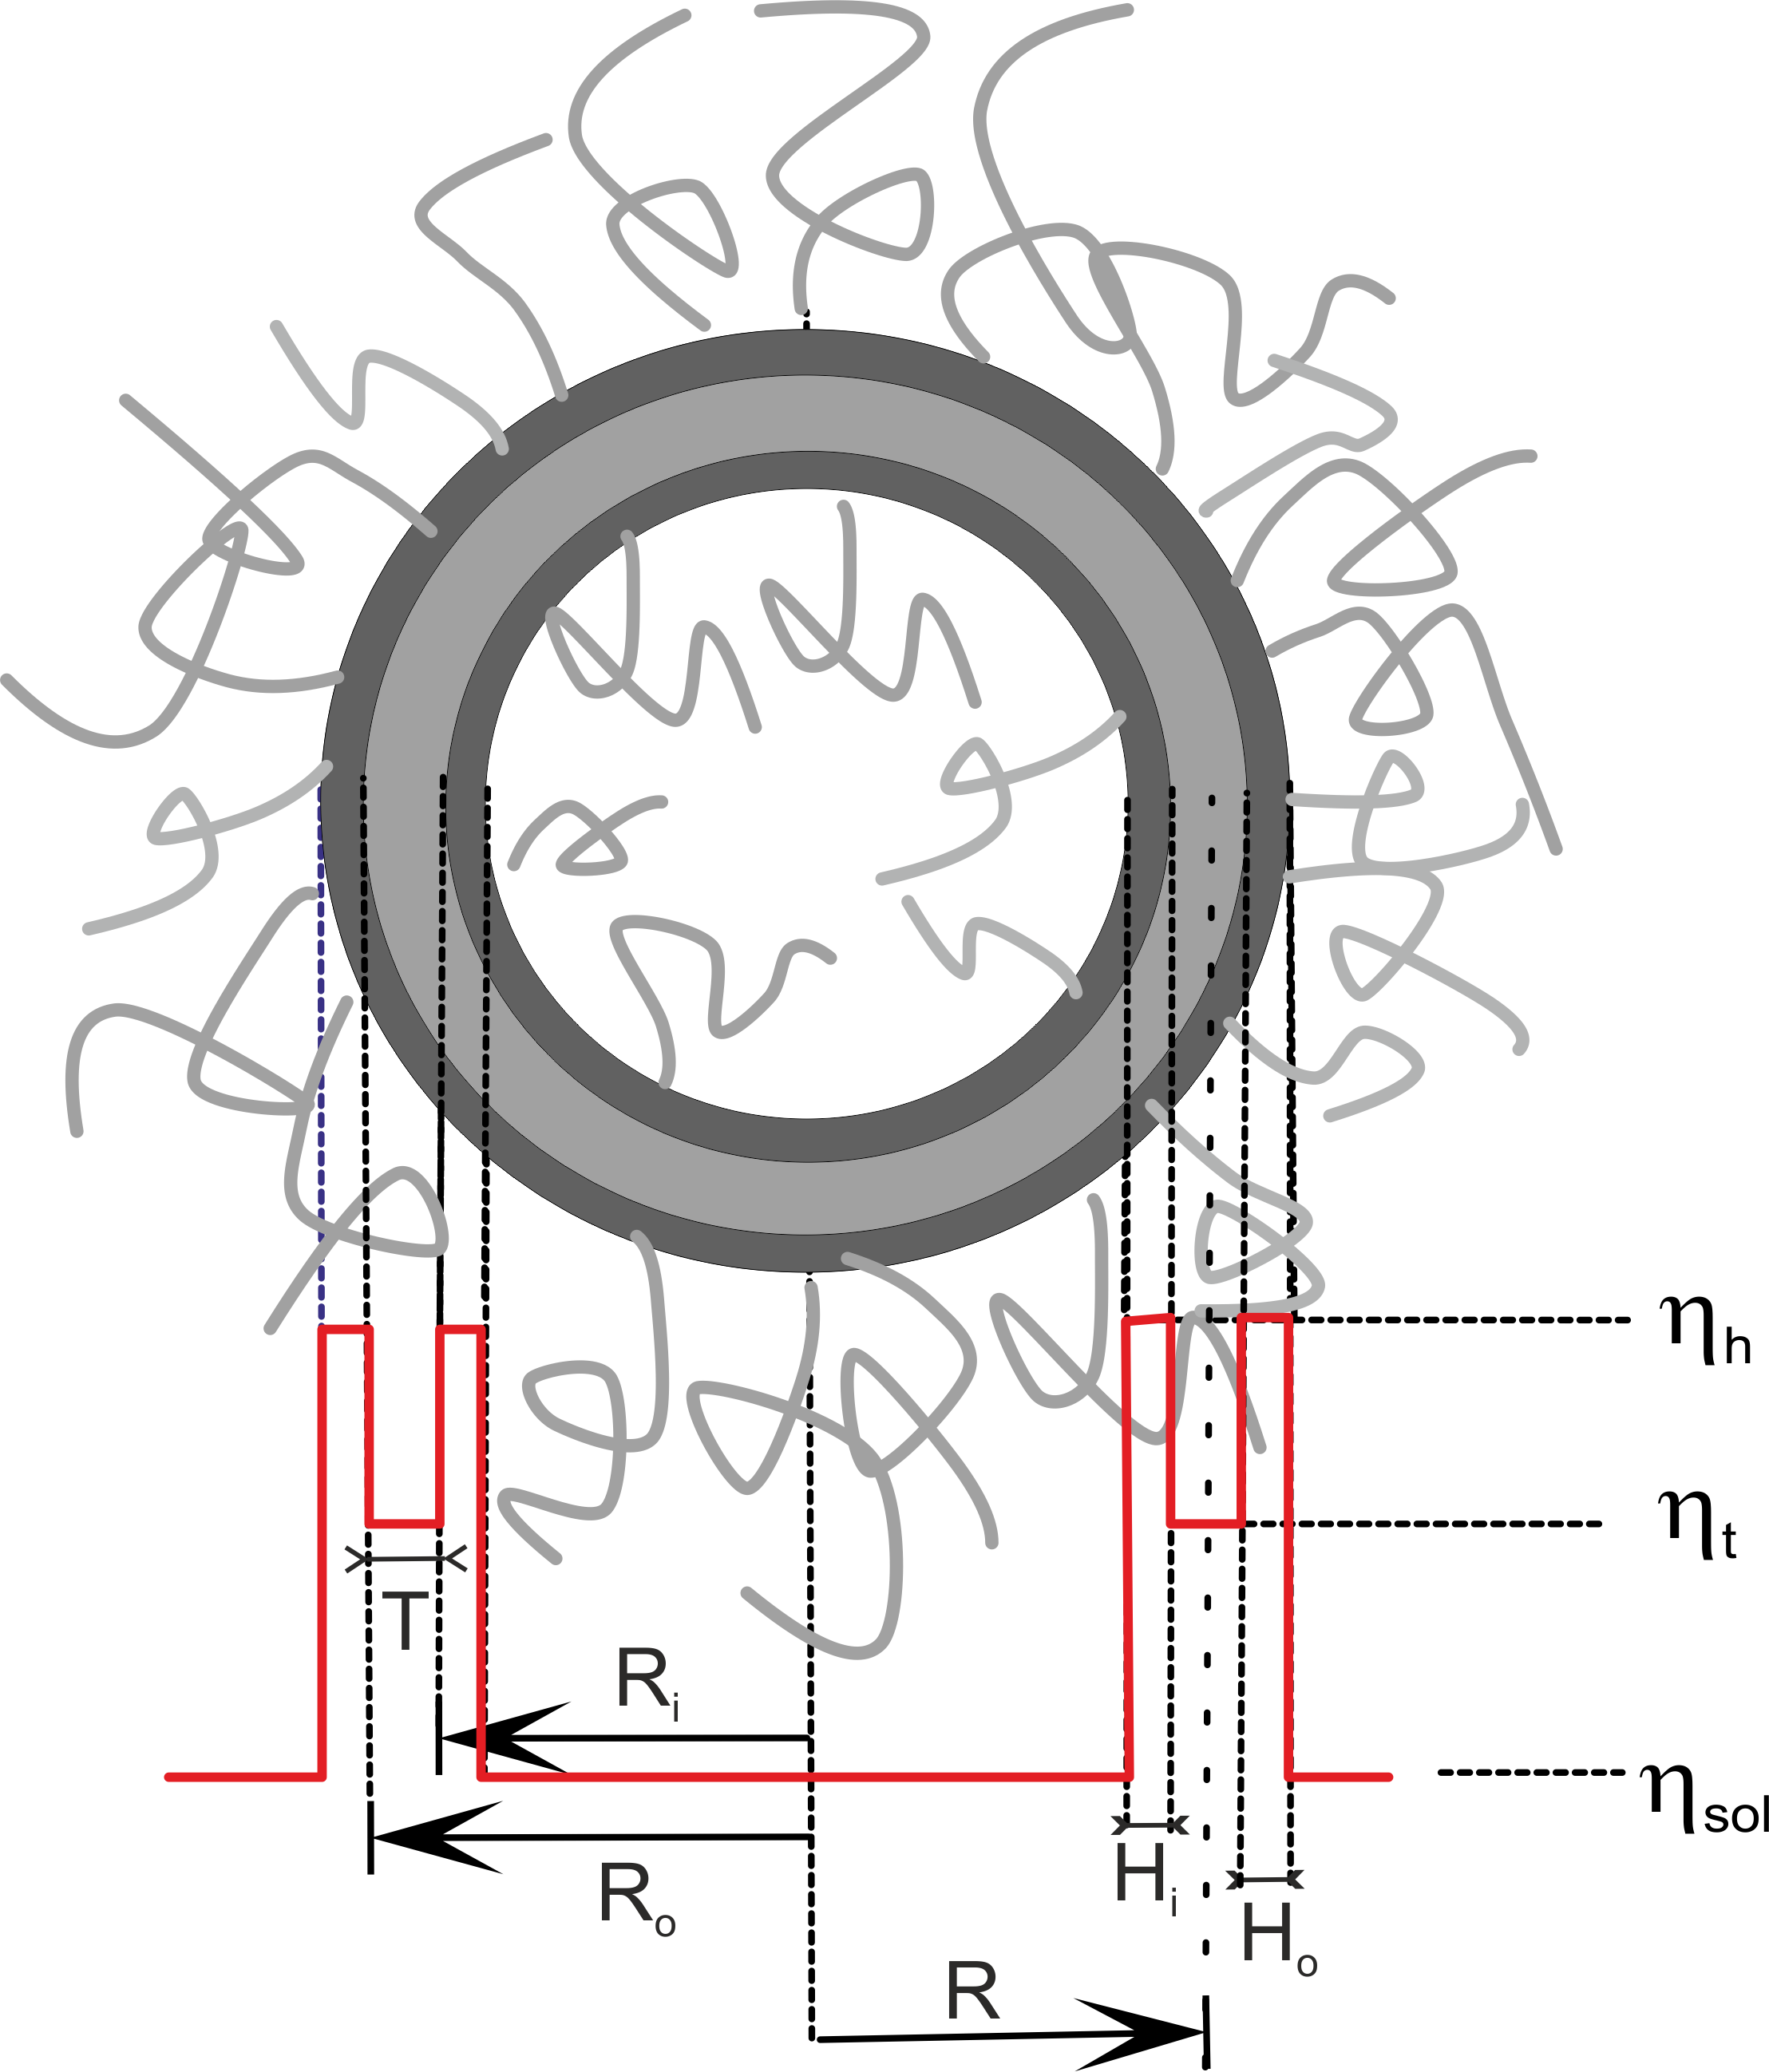
\includegraphics[width=0.7\textwidth]{../images/form_factor/vesicles/vesiclePEGpiecewconst.png}
\end{center}
\caption{scheme of PEGylated vesicle with PEG molecules attached in as well outside the vesicle but otherwise a piecewise constant scattering cross section of the membrane}
\label{fig:vesiclePEGpiecewconst}
\end{figure}

These parameters now needs to be expressed by known properties of the involved macro molecules. Scattering length densities are typically calculated from the known chemical sum formula and the bulk density of the molecules. The sum formula allows to calculated the molecular mass as well as the overall scattering length of the molecule, which then would allow to calculate the scattering length density of the molecule. However, in a solvent the molecular volume might change. Therefore volumetric measurements of the molecular volume in the used solvent are more precise and preferable, if available. Also literature values for the molecular volume of the head group $V_\mathrm{h}$ separated from the molecular volume of the tail group $V_\mathrm{t}$ are available.

These molecular volumes then can be used to determine the number of lipids per vesicle and the relative volume of the head group shells and the tail core in the membrane layer. If the thickness $T$ of the tail group layer and the radius of the vesicle $R$ are given the other quantities can be calculatred by
\begin{align}
R_\mathrm{i} &= R-\frac T2 \\
R_\mathrm{o} &= R+\frac T2 \\
n_\mathrm{l,i} &= \frac43 \frac{\pi}{V_\mathrm{t}} \left(R^3-R_\mathrm{i}^3\right) \\
n_\mathrm{l,o} &= \frac43 \frac{\pi}{V_\mathrm{t}} \left(R_\mathrm{o}^3-R^3\right) \\
V_\mathrm{v,h,i} &= n_\mathrm{l,i} V_\mathrm{h} \\
V_\mathrm{v,h,o} &= n_\mathrm{l,o} V_\mathrm{h} \\
n_\mathrm{i} &= n_\mathrm{l,i} f_\mathrm{PEG,i} \\
n_\mathrm{o} &= n_\mathrm{l,o} f_\mathrm{PEG,o} \\
H_\mathrm{i} & =  R - \frac T2 - \frac12 \left[\left(2R-T\right)^3 - \left(12R^2T-6RT^2+T^3\right)\frac{V_\mathrm{h}}{V_\mathrm{t}}\right]^{1/3} \\
H_\mathrm{o} & = -R - \frac T2 + \frac12 \left[\left(2R+T\right)^3 + \left(12R^2T+6RT^2+T^3\right)\frac{V_\mathrm{h}}{V_\mathrm{t}}\right]^{1/3}
\end{align}
Further model input parameters are the fraction of lipids decorated with PEG inside the vesicle $f_\mathrm{PEG,i}$ and outside the vesicle  $f_\mathrm{PEG,o}$.
In this model it is assumed that neither the tail layer nor the head group layers contain any solvent. The distance of the center of mass for the attached PEG molecules is assumed to be equal to its radius of gyration $R_g$.
~\\
\subsubsection{PEGylated liposome with smeared scattering length density profile} ~\\

In practise it could be shown \cite{Pabst2002,Brzustowicz2005} that at least for x-rays the scattering length density profiles across a membrane are better modelled by a smooth transition and gaussian scattering length density profile have been suggested and successfully been used. However, using Gaussian profiles the use of known molecular parameters like molecular volume are not so straight forward to be integrated as constrains for the input parameters.
Here we therefore introduce a smooth transition between the scattering length density of the hydrocarbon chain and the phospholipid head group as well as between the head group and the solvent. The transition can be performed with any sigmoidal function which smoothly varies between 0 and 1. In practice all cumulative distribution functions are such functions and are therefore typically used for this task are
\begin{align}
  w_\mathrm{logistic}(x) &=\frac{1}{1+\exp(-x)} \\
  w_\mathrm{Laplace}(x) &= \begin{cases}
                             \frac12 \exp(x), & \mbox{if } x\geq 0 \\
                             1-\frac12 \exp(-x), & \mbox{otherwise}.
                           \end{cases}  \\
  w_\mathrm{Cauchy}(x) &= \frac{1}{\pi}\arctan(x)+\frac12  \\
  w_\mathrm{Normal}(x) &=\frac12 \left[1+\operatorname{erf}(x/\sqrt{2})\right]  \\
  w_\mathrm{Rayleigh}(x) &= \begin{cases}
                             0, & \mbox{if } x\leq 0 \\
                             1-\exp\left(-x/\sqrt{2}\right), & \mbox{otherwise}.
                           \end{cases} \\
  w_\mathrm{algebraic}(x) &=\frac12 + \frac12 \frac{x}{\sqrt{1+x^2}} \qquad\mbox{algebraic transition function}\\
  w_\mathrm{Fermi}(x) &=1-\frac{1}{1+\exp(x)} \\
  w_\mathrm{Gudermannian}(x) &=\frac{2}{\pi}\arctan\left(\tanh(x/2)\right)+\frac12\\
  w_\mathrm{tanh}(x) &=\frac12 + \frac12 \tanh(x)
\end{align}
These transition function are here used to describe the rise and fall of the scattering length density profiles at interfaces.
The scattering length density profile $\eta_{\mathrm{l},i}(x)$ of layer $i$ is then given by
\begin{align} \label{eq:thinlayersprofile}
  \eta_{\mathrm{l,type},i}(x) &=  \left(\eta_i-\eta_\mathrm{sol}\right) w_{\mathrm{type},i}\left(\frac{x-R_{i}}{\sigma_{i}}\right)  \left[1- w_{\mathrm{type},i+1}\left(\frac{x-R_{i+1}}{\sigma_{i+1}}\right)\right]
\end{align}
The falling profile $\left[1- w_{\mathrm{type},i+1}\left(\frac{x-R_{i+1}}{\sigma_{i+1}}\right)\right]$ of the $i^\mathrm{th}$-layer is assumed being of the same type and with the same input parameters as the rising profile $w_{\mathrm{type},i+1}\left(\frac{x-R_{i+1}}{\sigma_{i+1}}\right)$ of the $(i+1)^\mathrm{th}$-layer. By this we assume within the overlap region a mixture of the elements of both layers, with a smooth transition.

The scattering intensity for a smoothed profile contains the same contribution as for a piecewise constant profile according to equation \ref{eq:vesicePEGsphsh}. However, the scattering contribution $I_\mathrm{vv}(q)$, as well as $I_\mathrm{vi}(q)$ $I_\mathrm{vo}(q)$ from the lipid vesicle needs to be calculated of layers with a smooth scattering length density profile according to eq.\ \ref{eq:thinlayersprofile}. In the following we use $w_\mathrm{Laplace}(x)$ as for such a profile all needed Fourier transformations can be calculated analytically.
\begin{figure}[htb]
\begin{subfigure}[b]{.48\textwidth}
   \centering
    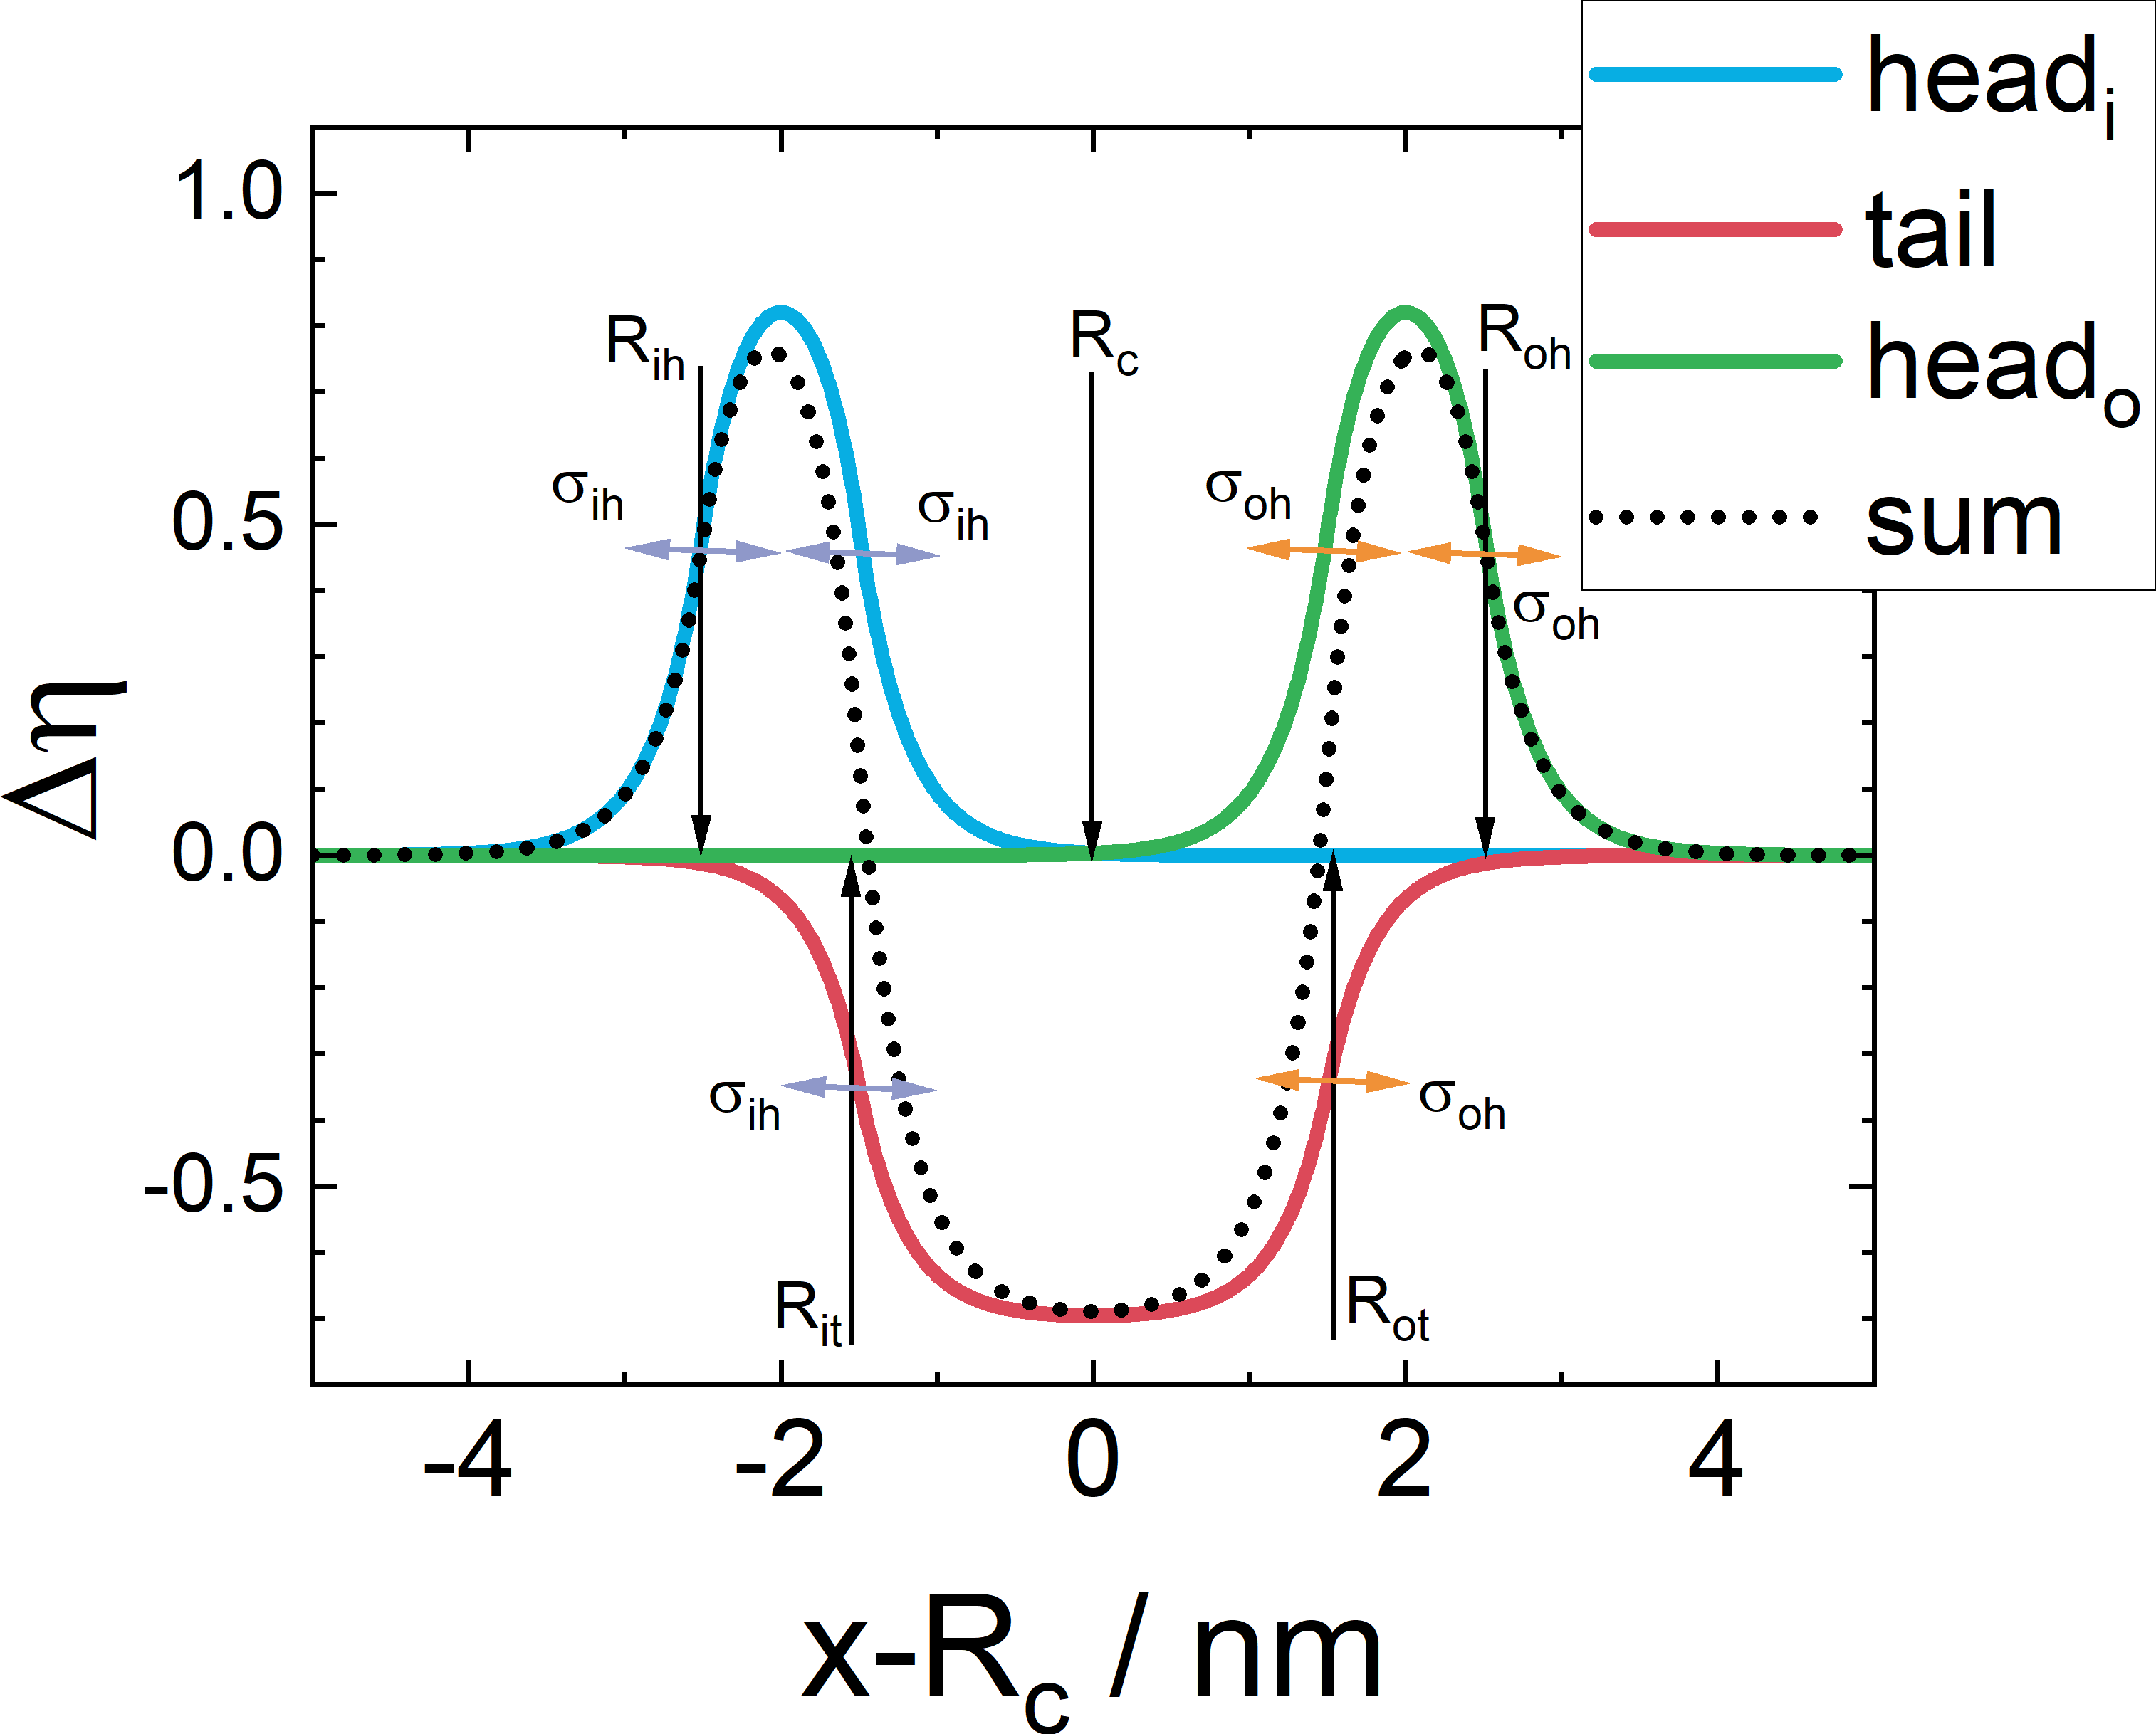
\includegraphics[width=\textwidth]{../images/form_factor/vesicles/vesicle_profile1.png}
    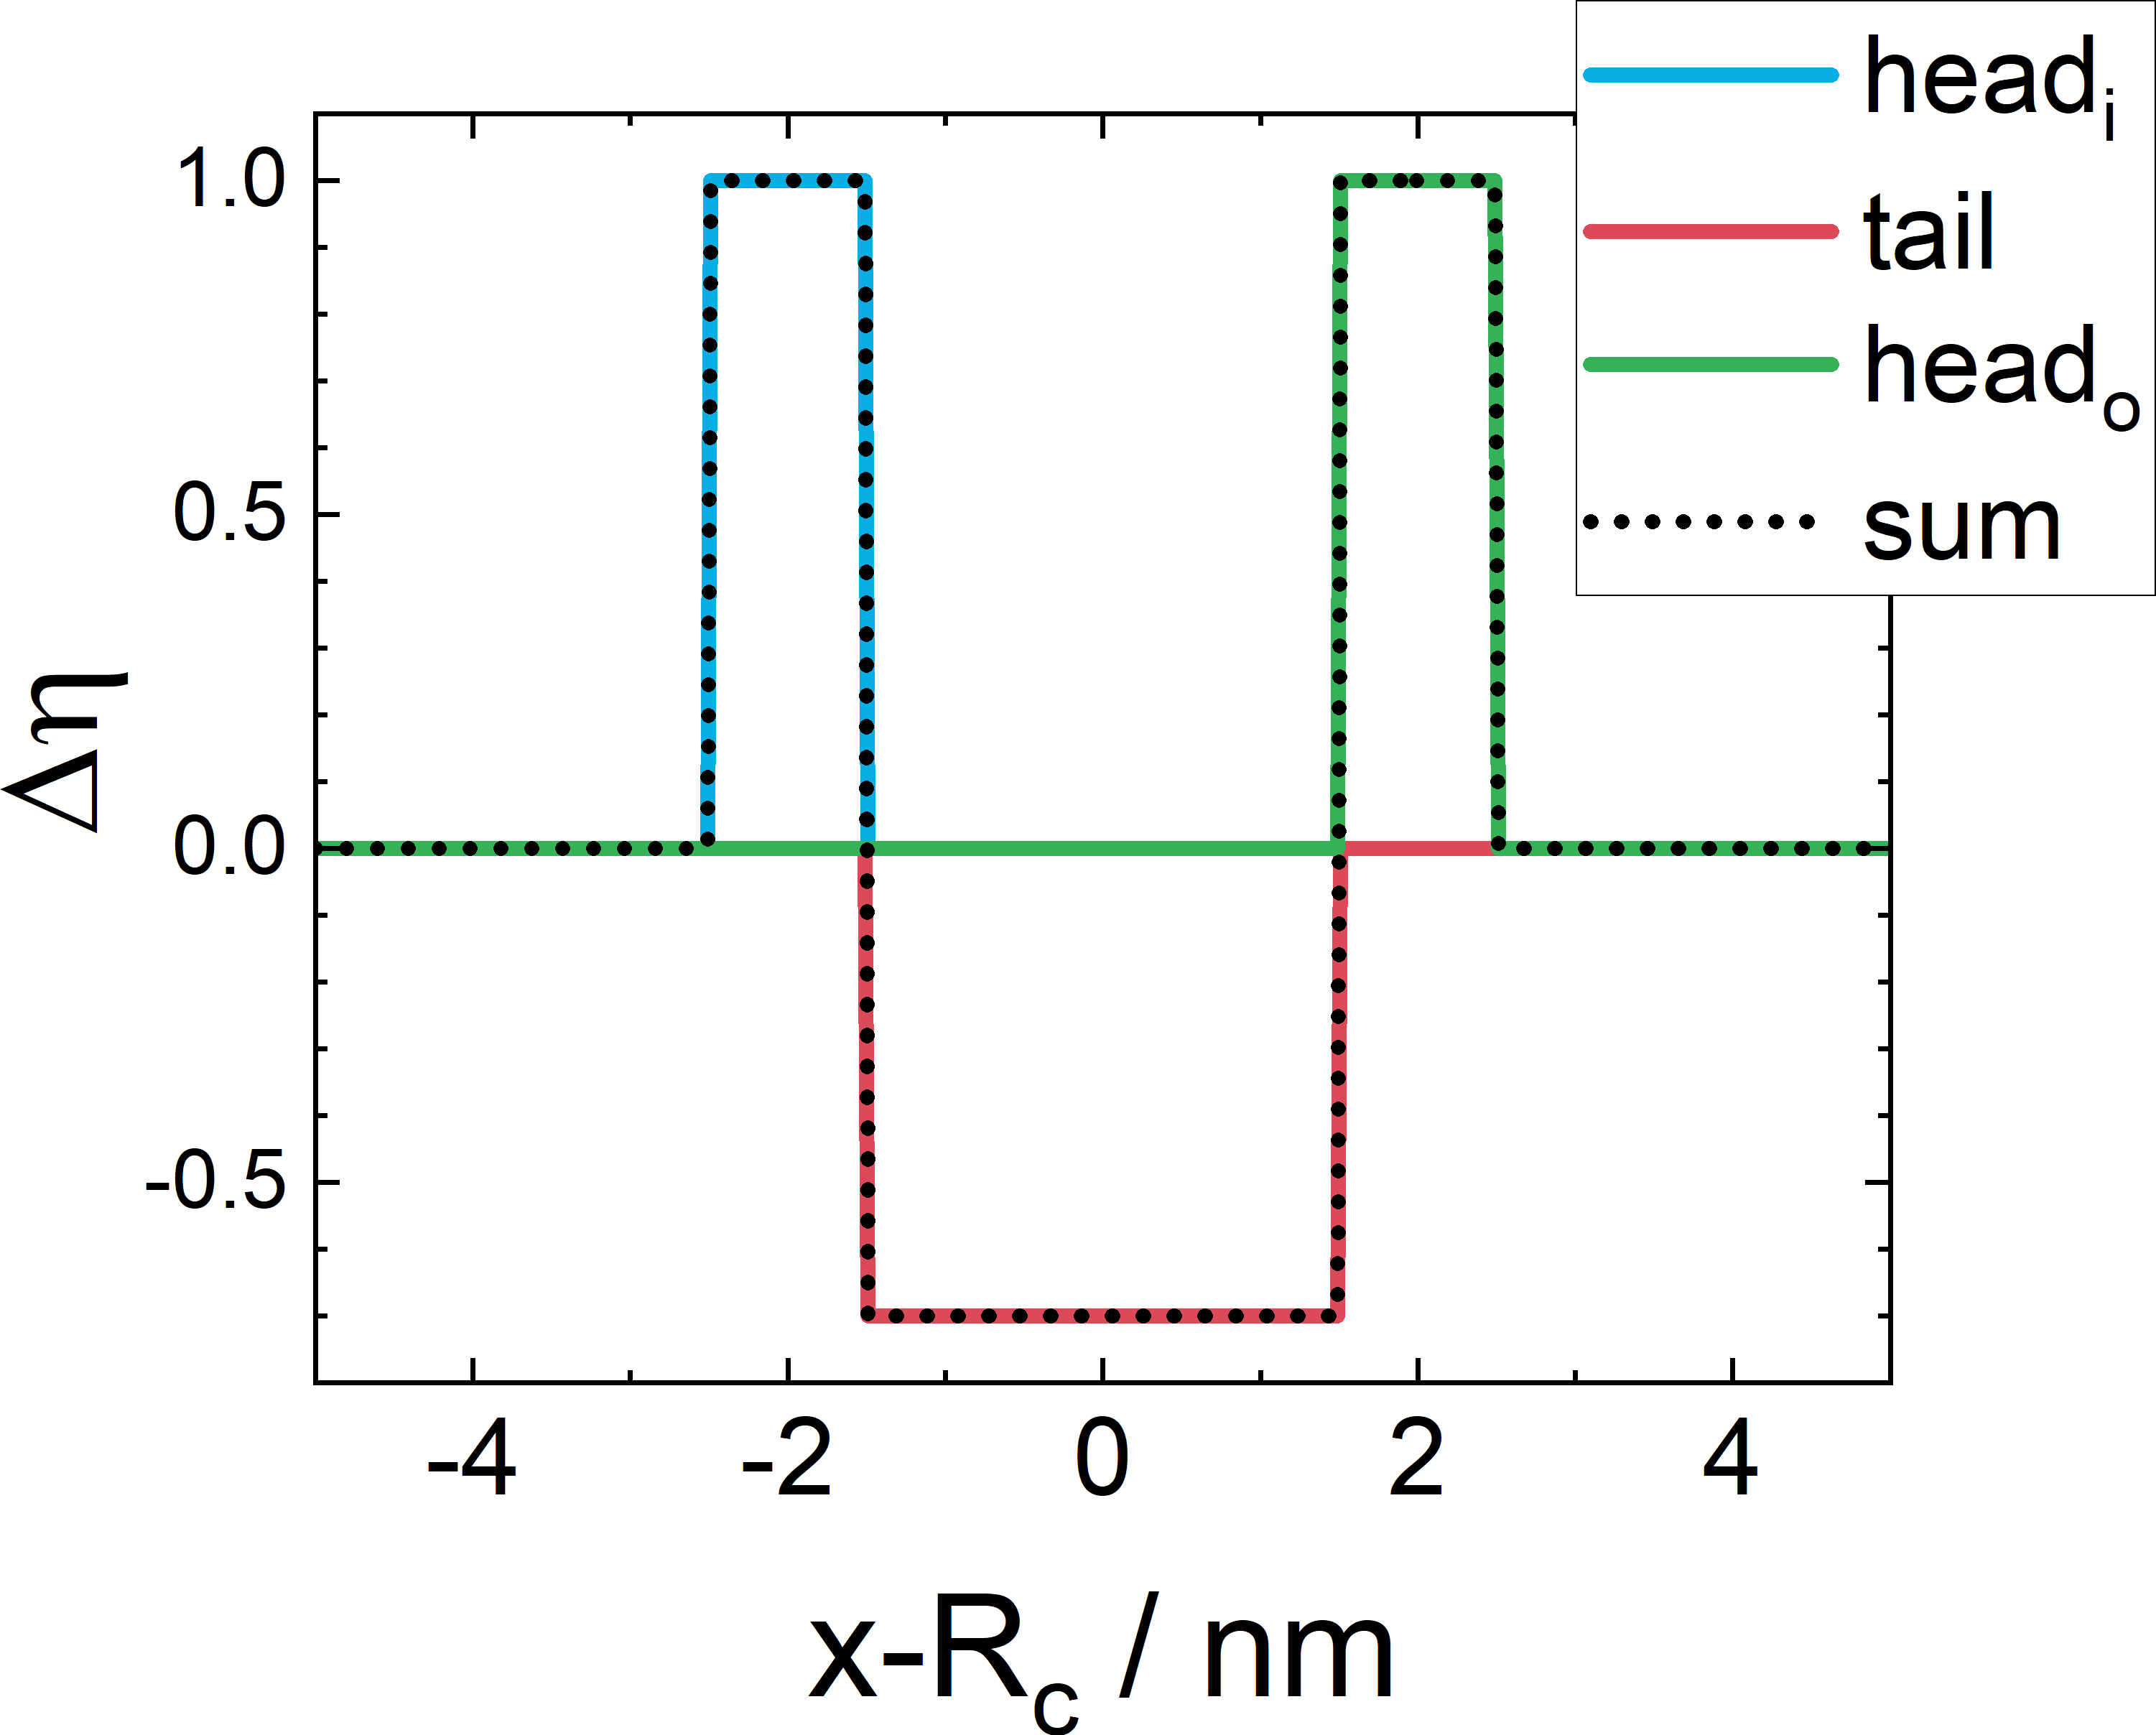
\includegraphics[width=\textwidth]{../images/form_factor/vesicles/vesicle_profile2.png}
   \caption{head groups with positive contrast and tail group with negative contrast relative to solvent. Top picture is calculated with smeared interfaces and bottom one with sharp interfaces.}
   \label{fig:vesicle_profile12}
\end{subfigure}
\hfill
\begin{subfigure}[b]{.48\textwidth}
   \centering
    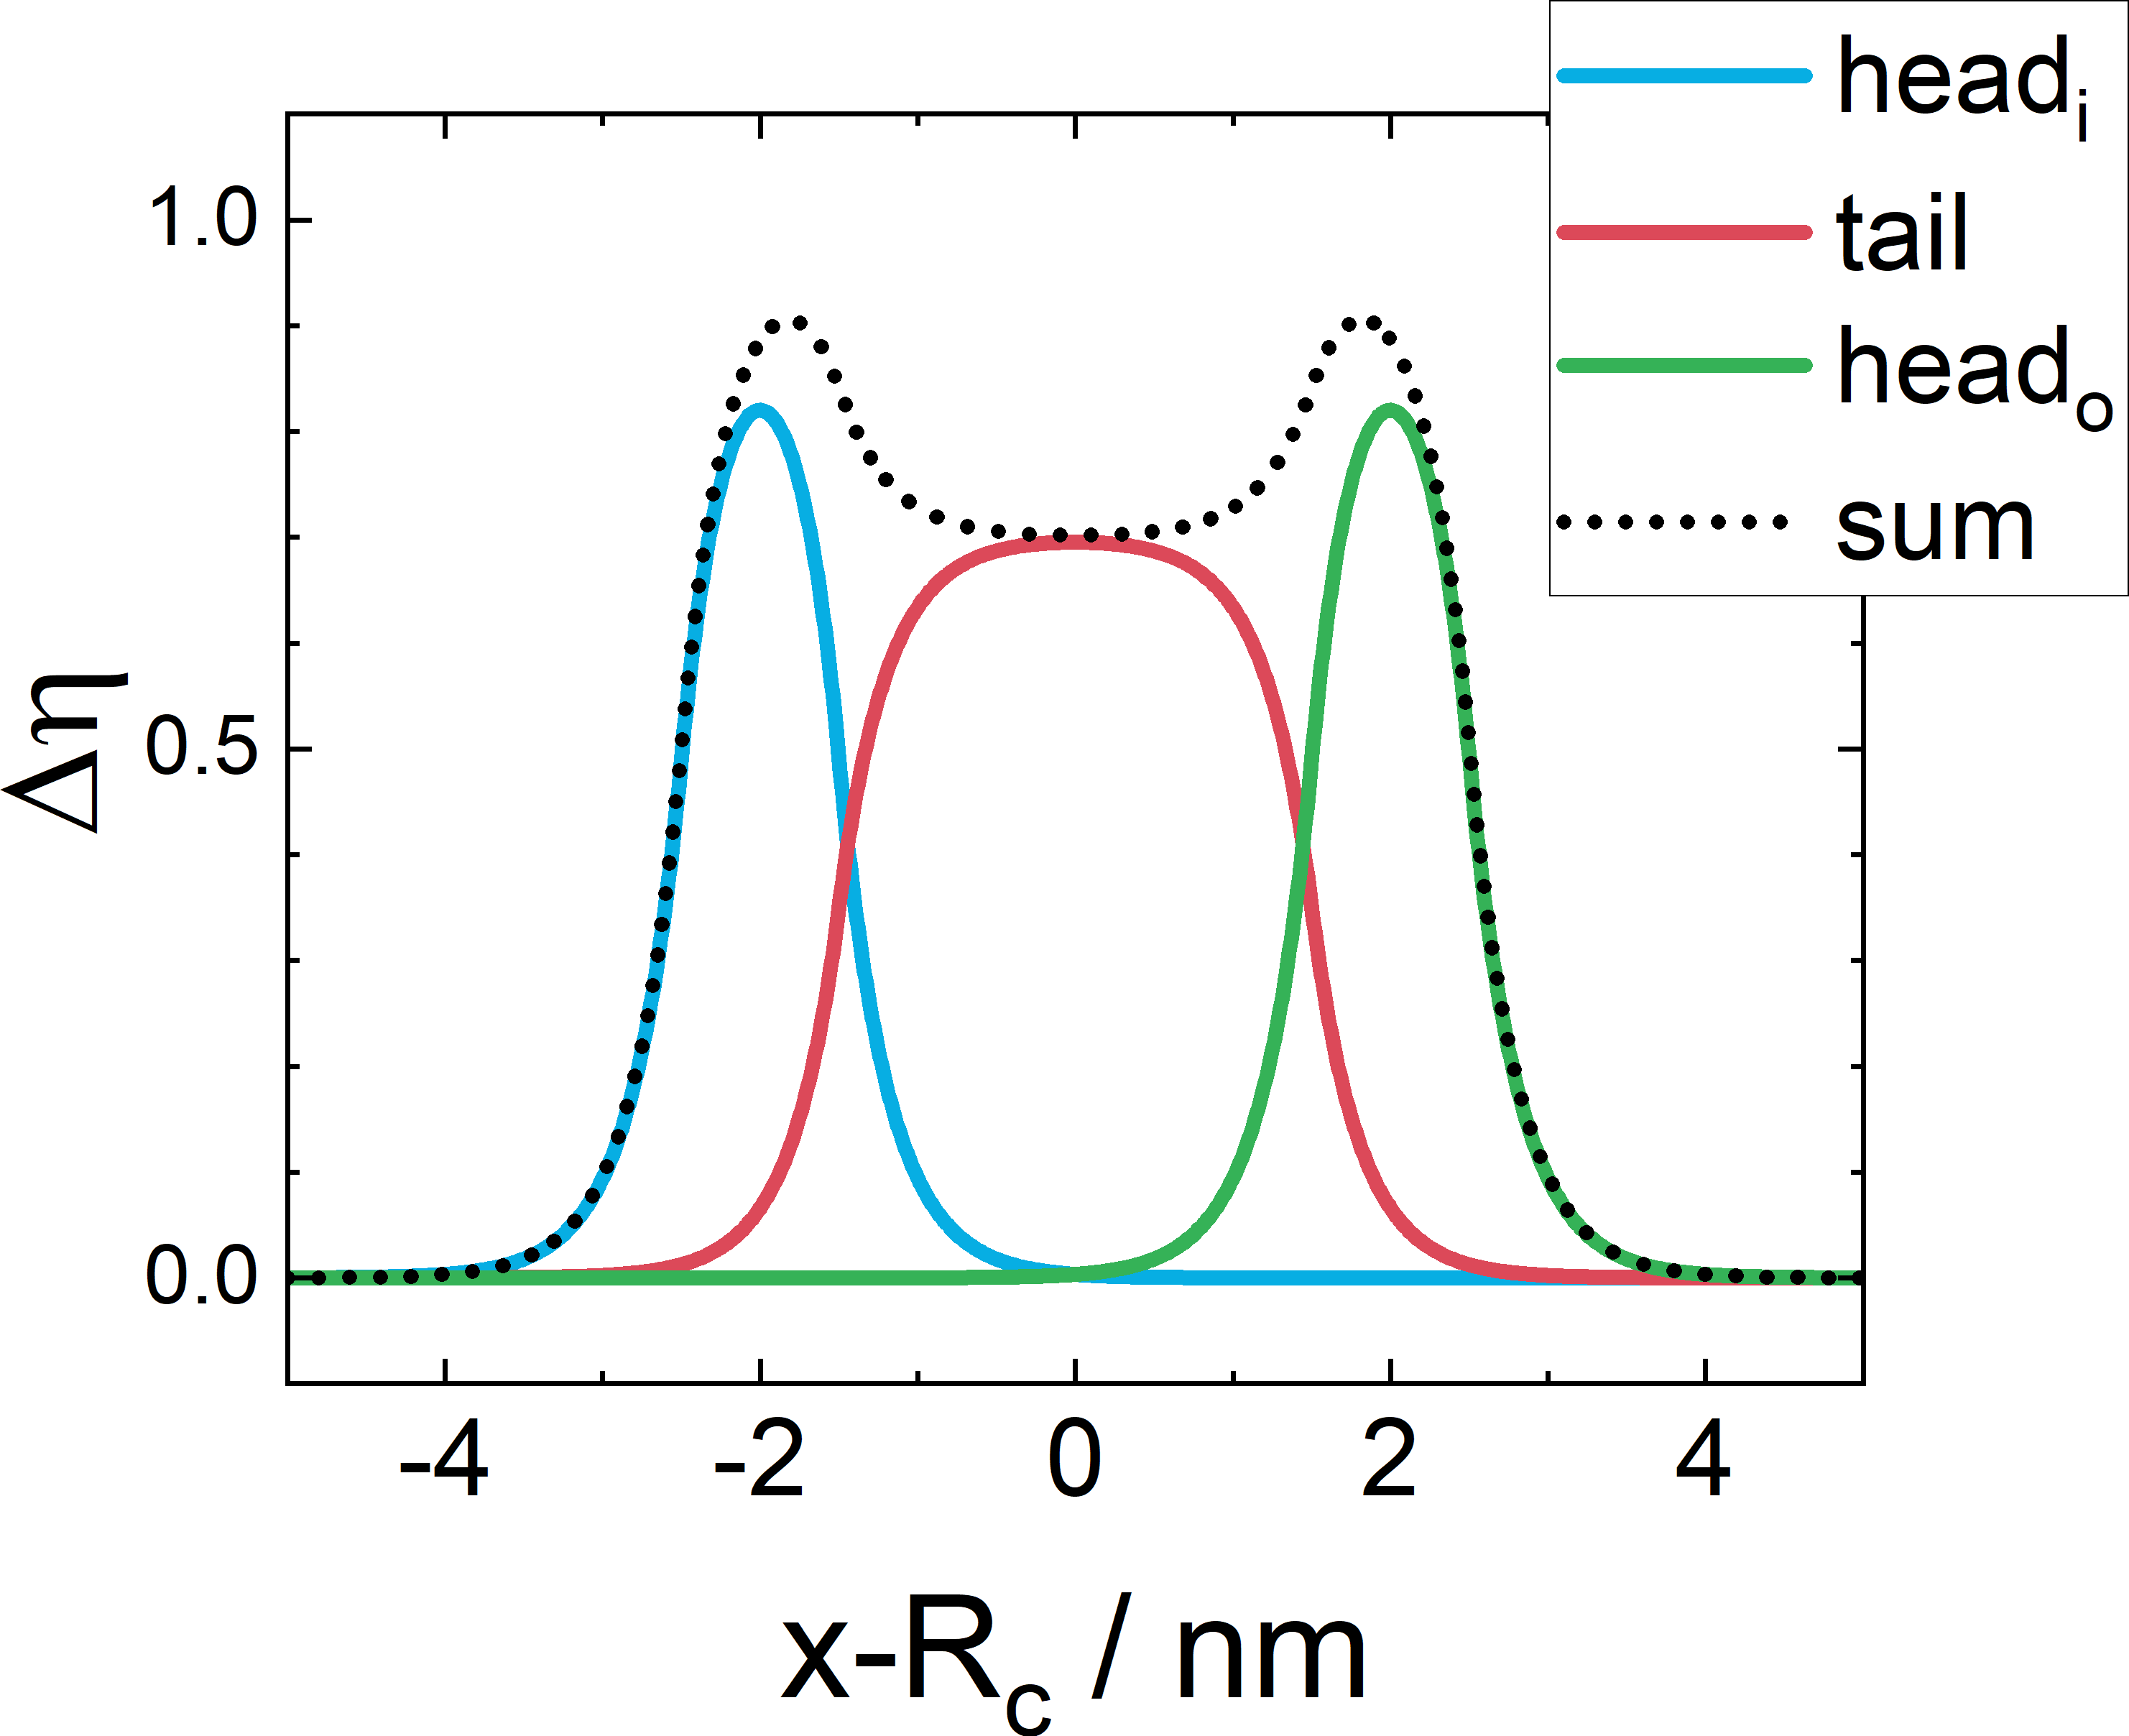
\includegraphics[width=\textwidth]{../images/form_factor/vesicles/vesicle_profile3.png}
    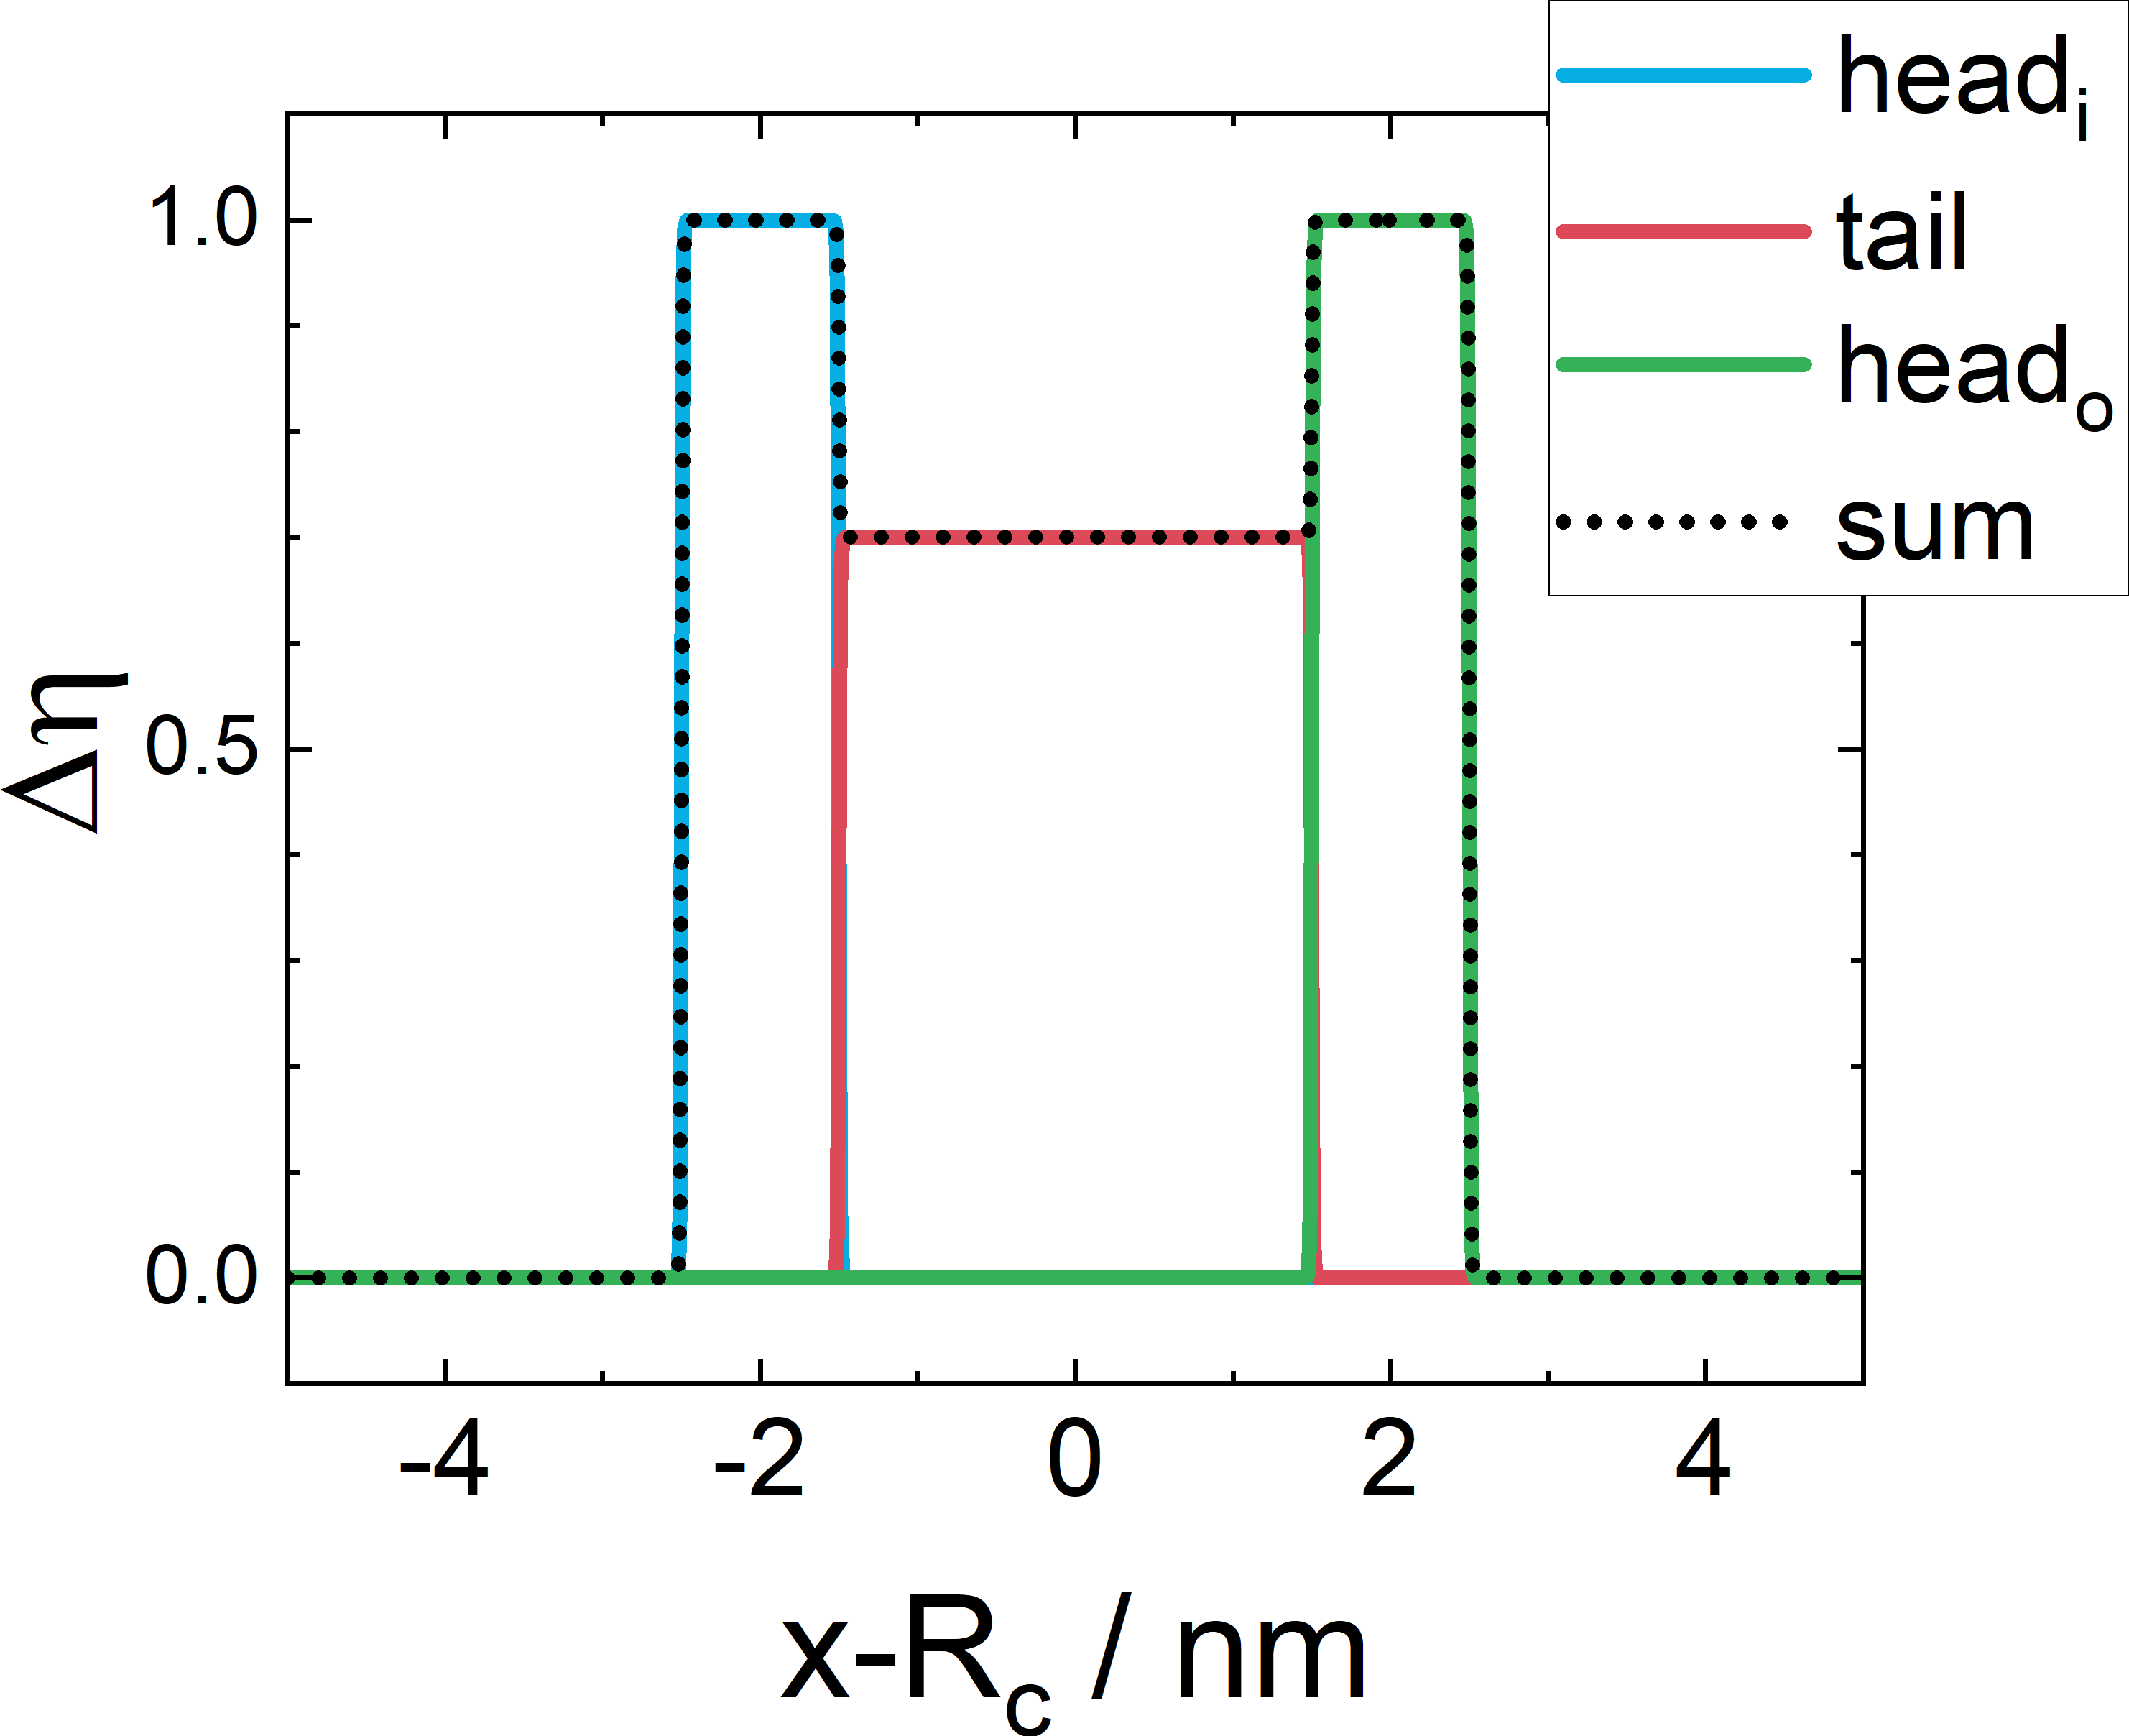
\includegraphics[width=\textwidth]{../images/form_factor/vesicles/vesicle_profile4.png}
   \caption{head and tail group have both positive contrast relative to solvent.Top picture is calculated with smeared interfaces and bottom one with sharp interfaces.}
   \label{fig:vesicle_profile34}
\end{subfigure}
\caption{scattering length density profiles across liposome membrane} \label{fig:vesicle_profiles}
\end{figure}
The scattering length density profile of a lipid bilayer $\eta_\mathrm{bilayer}(r)$ then reads as
\begin{align}\label{eq:eta_bilayer_smoothed}
  \eta_\mathrm{bilayer}(r) & =  \eta_{\mathrm{l,Laplace},ih}(r,\sigma_{ih},R_{ih},\sigma_{ih},R_{it},\eta_h,\eta_\mathrm{sol}) \nonumber \\
   & \qquad + \eta_{\mathrm{l,Laplace},t}(r,\sigma_{ih},R_{it},\sigma_{oh},R_{ot},\eta_t,\eta_\mathrm{sol}) \\
   & \qquad + \eta_{\mathrm{l,Laplace},oh}(r,\sigma_{oh},R_{ot},\sigma_{oh},R_{oh},\eta_h,\eta_\mathrm{sol}) \nonumber
\end{align}
The scattering amplitude is the Fourier transform of this profile
\begin{align}
  F_\mathrm{bilayer}(q) &=  \int_0^{\infty} 4\pi r^2  \eta_\mathrm{bilayer}(r) \frac{\sin qr}{qr}\mathrm{d}r
\end{align}
and can be performed fully analytically but is quite lengthy and has been obtained by a symbolic algebra software \cite{Mathematica_12_1}. The overall volume of the tail groups as well as those of the headgroups in and outside the vesicles are obtained by integrating \ref{eq:thinlayersprofile} and using a scattering length density contrast of 1
\begin{align}\label{eq:V_of_thinlayersprofile}
  V_{ih} &=  \int_0^{\infty} 4\pi r^2  \eta_{\mathrm{l,Laplace},ih}(r) \mathrm{d}r \\
  V_{t}  &=  \int_0^{\infty} 4\pi r^2  \eta_{\mathrm{l,Laplace},t}(r)  \mathrm{d}r \\
  V_{oh} &=  \int_0^{\infty} 4\pi r^2  \eta_{\mathrm{l,Laplace},oh}(r) \mathrm{d}r
\end{align}
As the form factor is parameterized in terms of the molecular volume of the head $V_\mathrm{head}$ and tail $V_\mathrm{tail}$ groups of a lipid molecule the following constrains needs to be fulfilled
\begin{align}
  \frac{V_{ih}}{\frac12 V_{t}} &= \frac{V_\mathrm{head}}{V_\mathrm{tail}} \\
  \frac{V_{oh}}{\frac12 V_{t}} &= \frac{V_\mathrm{head}}{V_\mathrm{tail}}
\end{align}
This is done by adapting the head group layer widths $H_{i}$ and $H_{o}$ using a root finding algorithm. Hereby $H_{i}= R-R_{i}$ and $H_{o}=R_{o}-R$ according to the sketch in fig.\ \ref{fig:vesiclePEGpiecewconst}.

\vspace{5mm}
\hspace{1pt}\\
\uline{Input Parameters for model \texttt{BilayeredVesicle}:}\\
\begin{description}
\item[\texttt{R}] vesicle radius $R$ (center of vesicle to center of lipid bilayer)
\item[\texttt{sigma\_R}] size distribution width parameter $\sigma_{R}$
\item[\texttt{T}] thickness of centrail tail layer $T$
\item[\texttt{sigma\_T}] size distribution width parameter $\sigma_T$
\item[\texttt{sigma\_i}] smearing width parameter of membrane interface inside vesicle
\item[\texttt{sigma\_o}] smearing width parameter of membrane interface outside vesicle
\item[\texttt{Rg}] radius of gyration of attached PEG molecules
\item[\texttt{f\_PEG\_i}] fraction of PEG decorated inner lipids where PEG is pointing towards inside of vesicle
\item[\texttt{f\_PEG\_o}] fraction of PEG decorated outer lipids where PEG is pointing towards outside of vesicle
\item[\texttt{V\_PEG}] molecular volume of PEG $V_\text{PEG}$
\item[\texttt{eta\_PEG}] scattering length density of PEG $\eta_\text{PEG}$
\item[\texttt{V\_head}] molecular volume of lipid head group $V_\text{h}$
\item[\texttt{eta\_head}] scattering length density of lipid head group $\eta_\text{h}$
\item[\texttt{V\_tail}] molecular volume of lipid tail group $V_\text{t}$
\item[\texttt{eta\_tail}] scattering length density of lipid tail group $\eta_\text{t}$
\item[\texttt{eta\_sol}] scattering length density of solvent $\eta_\text{sol}$
\end{description} 